\documentclass[10pt]{article}
\oddsidemargin -.2in
\evensidemargin -.2in
\topmargin -.2in
\textwidth 6.9in
\textheight 8.7in
%%%%%%%%%%%%%%%%%%%%%%%%%

\usepackage[parfill]{parskip}    % Activate to begin paragraphs with an empty line rather than an indent
\usepackage{latexsym, amssymb, bbm}
\usepackage{amsmath}
\usepackage{amsfonts}
\usepackage{amsthm}
\usepackage{verbatim}
\usepackage{fancyhdr}
\usepackage{enumerate}
\usepackage{mathtools}
\usepackage{graphicx}
\usepackage{float}
\usepackage[linesnumbered,vlined]{algorithm2e}
\SetEndCharOfAlgoLine{}
\usepackage{changepage}

%%%%%%%%%%%%%%%%%%%%%%%%%

\newtheorem{thm}{Theorem}[section]
\newtheorem{lem}[thm]{Lemma}
\newtheorem{prop}[thm]{Proposition}
\newtheorem{cor}[thm]{Corollary}
\newtheorem{cla}[thm]{Claim}
\newtheorem{con}[thm]{Conjecture}

\theoremstyle{definition}
\newtheorem*{defn}{Definition}
\newtheorem{example}[thm]{Example}
\newtheorem{axiom}{Axiom}
\newtheorem*{note}{Note}
\newtheorem*{question}{Question}

\theoremstyle{remark}
\newtheorem{case}{Case}

%%%%%%%%%%%%%%%%%%%%%%%%%
%%%%%%%%%%%%%%%%%%%%%%%%%%
%%%%%%%% EDIT HERE %$%%%%%%%%%
%%%%%%%%%%%%%%%%%%%%%%%%%%%%
%%%%%%%%%%%%%%%%%%%%%%%%%%%%%

\newcommand{\classname}{Multiple Testing, Modern Inference, and Replicability}
\newcommand{\classnumber}{STAT 27850}
\newcommand{\due}{3 March 2017}
\newcommand{\num}{Gerrymandering}
\newcommand{\type}{Final Project}

%%%%%%%%%%%%%%%%%%%%%%%%%%%%%
%%%%%%%%%%%%%%%%%%%%%%%%%%%%
%%%%%%%%%%%%%%%%%%%%%%%%%%%
%%%%%%%%%%%%%%%%%%%%%%%%%%
%%%%%%%%%%%%%%%%%%%%%%%%%


%-------------------------------------------------------


%-------------------------------------------------------

\newcommand{\lecture}[1]{\centerline{\fbox{\textbf{#1}}}}
\newcommand{\que}[2] {\vspace{.25in} \fbox{#1} #2 \vspace{.10in}}
\renewcommand{\part}[1] {\vspace{.10in} {\bf (#1)}}


%%%%%%%%%%%%%%%%%%%%%%%%%%

% SHORTCUTS FOR BLACKBOARD BOLD
\def\C{\mathbb{C}}
\def\N{\mathbb{N}}
\def\Q{\mathbb{Q}}
\def\R{\mathbb{R}}
\def\Z{\mathbb{Z}}
\def\1{\mathbbm{1}}
\def\P{\mathbb{P}}
\def\0{\emptyset}

% SHORTCUTS FOR MATH BOLD FONT
\def\ba{\mathbf{a}}
\def\bb{\mathbf{b}}
\def\be{\mathbf{e}}
\def\bm{\mathbf{m}}
\def\bh{\mathbf{h}}
\def\bu{\mathbf{u}}
\def\bw{\mathbf{w}}
\def\bv{\mathbf{v}}
\def\bS{\mathbf{\Si}}
\def\bmu{\boldsymbol{\mu}}
\def\bx{\mathbf{x}}
\def\by{\mathbf{y}}
\def\bz{\mathbf{z}}
\def\bzero{\mathbf{0}}
\def\bone{\mathbf{1}}

% SHORTCUTS FOR GREEK LETTERS
\def\a{\alpha}
\def\b{\beta}
\def\g{\gamma}
\def\G{\Gamma}
\def\d{\delta}
\def\D{\Delta}
\def\e{\varepsilon}
\def\k{\kappa}
\def\l{\lambda}
\def\m{\mu}
\def\r{\rho}
\def\s{\sigma}
\def\t{\tau}
\def\th{\theta}
\def\x{\xi}
\def\vp{\varphi}
\def\n{\nabla}
\def\w{\omega}
\def\z{\zeta}
\def\vp{\varphi}
\def\p{\phi}
\def\Ph{\Phi}
\def\L{\Lambda}
\def\Si{\Sigma}
\def\Th{\Theta}
\def\O{\Omega}

\def\el{\ell}

% SHORTCUTS FOR MATH SCRIPT
\def\sR{\mathscr{R}}
\def\sA{\mathscr{A}}
\def\sC{\mathscr{C}}
\def\sM{\mathscr{M}}
\def\sF{\mathscr{F}}
\def\sB{\mathscr{B}}
\def\sL{\mathscr{L}}

% SHORTCUTS FOR MATH CAPITALS
\def\A{\mathcal{A}}
\def\cC{\mathcal{C}}
\def\cE{\mathcal{E}}
\def\cF{\mathcal{F}}
\def\cH{\mathcal{H}}
\def\cL{\mathcal{L}}
\def\cM{\mathcal{M}}
\def\cP{\mathcal{P}}
\def\cU{\mathcal{U}}


\def\i{^{-1}}
\newcommand{\fin}{f^{-1}}
\def\lp{\mathop{\rm lp}}
\def\slp{\mathop{\rm slp}}
\def\ext{\mathop{\rm ext}}
\def\sep{\mathop{\rm sep}}
\def\rel{\mathop{\rm rel}}
\def\lub{\mathop{\rm lub}}
\def\glb{\mathop{\rm glb}}

\def\ds{\displaystyle}

\newcommand{\lpvar}[1]{\,\textrm{lp}_{#1}\,}
\newcommand{\ol}[1]{\overline{#1}}
\newcommand{\fl}[1]{\left\lfloor #1 \right\rfloor}
\newcommand{\cl}[2]{\left\lceil \frac{#1}{#2} \right\rceil}
\newcommand{\md}[1]{(\text{mod } #1)}
\newcommand{\cs}[1]{\begin{case} #1 \end{case}}
\newcommand{\abs}[1]{\left\lvert #1 \right\rvert}
\newcommand{\norm}[1]{\lVert#1\rVert}
\newcommand{\set}[1]{\{ #1 \}}
\DeclarePairedDelimiter{\ceil}{\lceil}{\rceil}
\DeclarePairedDelimiter{\floor}{\lfloor}{\rfloor}


\newcommand{\upint}[2]{
  \overline{\int_{#1}^{#2}}
}
\newcommand{\loint}[2]{
  \underline{\int_{#1}^{#2}}
}

\DeclareMathOperator{\spn}{span}
\DeclareMathOperator{\diam}{diam}
\DeclareMathOperator*{\E}{\mathbb{E}}
\DeclareMathOperator*{\pr}{\mathbb{P}}

\newenvironment{piecewise}{\left\lbrace
\begin{matrix}}
{
\end{matrix}
\right.
}



\def\defeq{\stackrel{\text{\tiny def}}=}

\def\la{\langle}
\def\ra{\rangle}

\def\ben{\begin{enumerate}}
\def\een{\end{enumerate}}

\def\ptl{\partial}
\newcommand{\pd}[2]{\frac{\ptl#1}{\ptl #2}}

\def\tb{\textbf}
\def\^{\wedge}
\def\del{\nabla}

% Little Stats things
\def\iid{\stackrel{iid}\sim}
\def\indep{\!\perp\!\!\!\perp}


% SHORTCUTS FOR LIMITS
\def\ltx{\lim_{t\to x}}
\def\lxp{\lim_{x\to p}}
\def\lxa{\lim_{x\to a}}
\def\lni{\lim_{n\to\infty}}
\def\lsni{\limsup_{n\to\infty}}
\def\lxi{\lim_{x\to\infty}}
\def\lxz{\lim_{x\to0}}
\def\lhz{\lim_{h\to0}}
\def\ltz{\lim_{t\to0}}

% SHORTCUTS FOR SUMMATIONS
\def\sion{\sum_{i=1}^n}
\def\sjon{\sum_{j=1}^n}
\def\sjom{\sum_{j=1}^m}
\def\sjod{\sum_{j=1}^d}
\def\sjok{\sum_{j=1}^k}
\def\snoi{\sum_{n=1}^\infty}
\def\sioi{\sum_{i=1}^\infty}
\def\snzi{\sum_{n=0}^\infty}
\def\snzN{\sum_{n=0}^N}
\def\skoi{\sum_{k=1}^\infty}
\def\siok{\sum_{i=1}^k}
\def\skon{\sum_{k=1}^n}
\def\skzn{\sum_{k=0}^n}
\def\pion{\prod_{i=1}^n}
\def\siod{\sum_{i=1}^d}


% SHORTCUTS FOR INTEGRALS
\def\ipp{\int_{-\pi}^\pi}
\def\iii{\int_{-\infty}^{\infty}}
\def\izp{\int_0^\pi}
\def\iztp{\int_0^{2\pi}}
\def\izr{\int_0^r}
\def\izo{\int_0^1}
\def\ioi{\int_1^\infty}
\def\iab{\int_a^b}
\def\izi{\int_0^\infty}
\def\riea{\sR(\a)}
\newcommand{\eval}[2]{\Big\vert_{#1}^{#2}}

% SHORTCUTS FOR ENVIRONMENTS
\newcommand{\al}[1]{\begin{align*}#1\end{align*}}
\newcommand{\aleq}[1]{\begin{equation}\begin{aligned}[b]#1\end{aligned}\end{equation}}
\newcommand{\bigb}[1]{\bigg(#1\bigg)}
\newcommand{\prf}[1]{\begin{proof}#1\end{proof}\vspace{3mm}}
\newcommand{\bmtx}[1]{\begin{bmatrix}#1\end{bmatrix}}
\newcommand{\enum}[2]{\begin{enumerate}[#1]#2\end{enumerate}}
\newcommand{\pwise}[1]{\begin{piecewise}#1\end{piecewise}}
\newcommand{\inm}[1]{\norm{#1}_2}
\newcommand{\enviro}[2]{\begin{#1}#2\end{#1}}
\newcommand{\tabler}[2]{\begin{center}\begin{tabular}{#1}#2\end{tabular}\end{center}}

\newcommand{\seq}[2]{\{#1_#2\}}
\DeclareMathOperator*{\argmin}{arg\,min}
\DeclareMathOperator*{\argmax}{arg\,max}

%%%%%%%%%%%%%%%%%%%%%%%%%%%%%%%%%%%%%%%%%%%%%%%%

\begin{document}
%--------------------------------------------------------------
\pagestyle{fancy}

\lhead{\classnumber}
\chead{\type:\space\num}
\rhead{\due}

\title{
    \vspace{-2cm}
	\classname \\
    \type: \num \\
    (Progress Report)
}
\author{
	 Peter Gao, Casper Neo, Nishesh Sharma
}
\date{
	\due\\
}

\maketitle
%--------------------------------------------------------------

\begin{enumerate}

    \item Motivations of a partisan re-district-er
    \begin{enumerate}

        \item A partisan incumbent will to try to win as many districts while
        still maintaining a margin of safety. To accomplish this goal the
        re-district-er will draw districts such that the other party's voters
        are concentrated in a few districts (voter packing) while their party's
        voters are spread out. The effect would be to win many districts with a
        narrow margin while losing few with large margins.


        \item Bipartisan re-district-er may want to increase stability and
        protect the incumbents. To accomplish this goal they will draw districts
        such that all incumbents win by margins large enough that their seat
        will not be contested.

        \item Something about the notion of stability

    \end{enumerate}

    \item Methods Implemented
    \begin{enumerate}
        \item Efficiency Gap (Stephanopoulos and McGhee 2015)

        Any votes cast towards a losing candidate is considered wasted. And
        all the votes cast towards a winning candidate in excess of the number
        of votes required to win is considered wasted.
        Let $wasted(A)$ be the number of wasted votes cast by party $A$.
        Then define the efficiency gap as
        $$
        \text{ Efficiency Gap}(A,B)\defeq \frac{wasted(A)-wasted(B)}{
        \#\text{votes}
        }
        $$

        \item Partisan Bias

        \item Lopsided Victories (Wang)

        If there is partisan gerrymandering then as evidence of voter packing,
        one party will win by large margins while the other party's
        will win by small margins. We use a two sided $T$ test to compare the
        means of the winning margin of the two parties. In order to deal with elections where one 
        party ran unopposed, we added an imputed value parameter that represents the assumed 
        percentage of votes that the winning party would have received had there been an opponent. 
        In most cases, tweaking this parameter's value does not significantly alter the p-value for 
        a given state and year. However, it is possible that across many years and many states, the 
        choice of imputed value is significant. We plotted the vote proportions in wins for both 
        Democrats and Republicans for many different states and years. Some sample graphs and p-
        values are displayed on the following page:  \\
        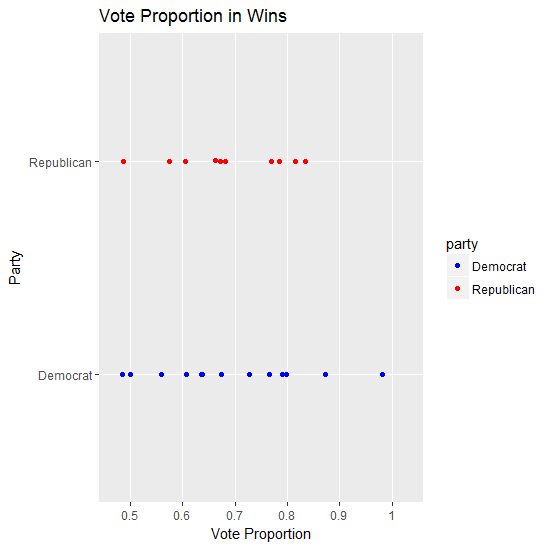
\includegraphics[scale=0.5]{PA1984}
        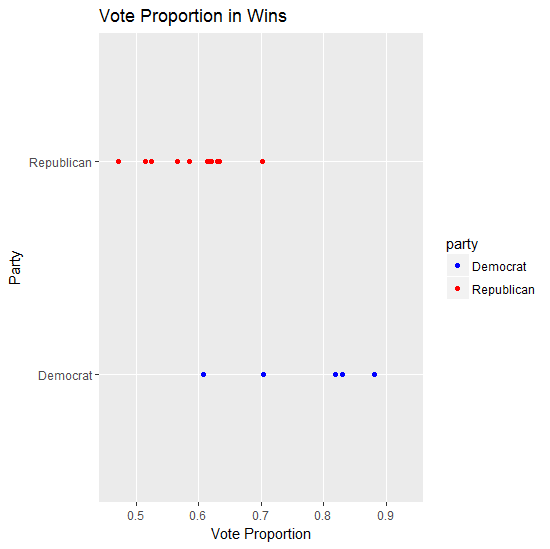
\includegraphics[scale=0.5]{PA2012} \\
        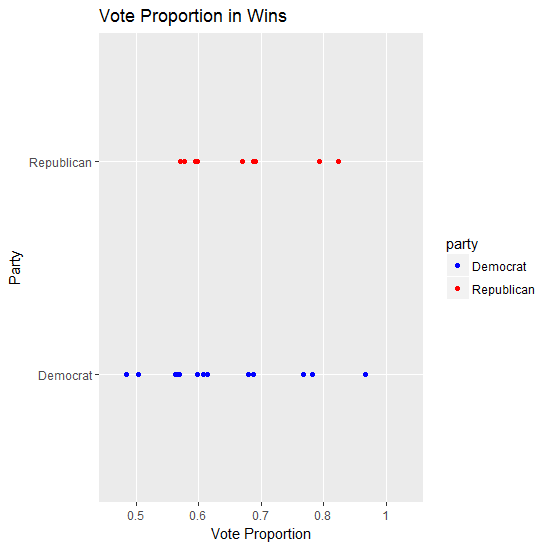
\includegraphics[scale=0.5]{IL1984}
        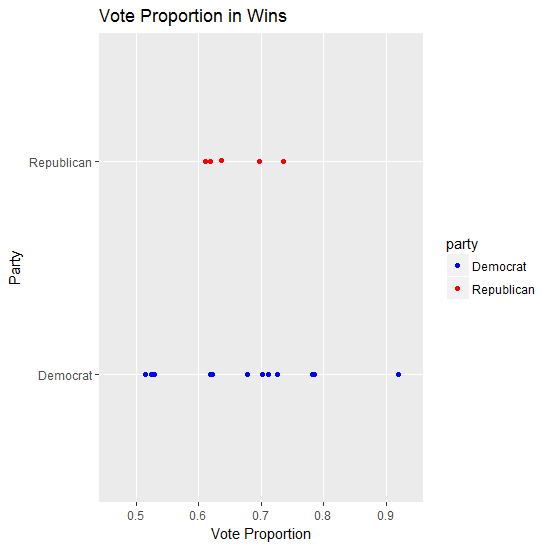
\includegraphics[scale=0.5]{IL2012} \\
        ~\\
        These graphs correspond to PA 1984 (p-value of 0.679), PA 2012 (p-value of 0.03), IL 1984 (p-value of 0.843), and IL 2012 (p-value of 0.766) respectively from left to right.

    \end{enumerate}
    \item Preliminary Results and challenges
    \begin{enumerate}
        \item One of the initial challenges was finding data.
        ``http://projects.iq.harvard.edu/eda/'' provides shape file and
        election data. However we found that the data formats were not uniform over
        different states (i.e. there were columns missing or named differently).
        ``https://www.ncsbe.gov/Election-Results'' provided data over just
        North Carolina. 


    \end{enumerate}

    \item Simulations (To be completed)
    \begin{enumerate}
        \item Sampling from Simulated Delegations - Excess seats (Wang)

        \item Perturbation of Existing Map

        For a given election outcome
        consider for $N$ simulations, exchanging $k$ voting blocks along the
        boundary of voting districts. If the original voting districts were
        gerrymandered we would expect our metrics to decrease in a majority of
        the simulations assuming the gerrymander-er would have, in
        gerrymandering, chosen a local maximum of our metrics by choice of map.

    \end{enumerate}
\end{enumerate}

%------------------------------------------------------------------------------------------------------------
\end{document}
